% Options for packages loaded elsewhere
\PassOptionsToPackage{unicode}{hyperref}
\PassOptionsToPackage{hyphens}{url}
%
\documentclass[
]{article}
\usepackage{lmodern}
\usepackage{amsmath}
\usepackage{ifxetex,ifluatex}
\ifnum 0\ifxetex 1\fi\ifluatex 1\fi=0 % if pdftex
  \usepackage[T1]{fontenc}
  \usepackage[utf8]{inputenc}
  \usepackage{textcomp} % provide euro and other symbols
  \usepackage{amssymb}
\else % if luatex or xetex
  \usepackage{unicode-math}
  \defaultfontfeatures{Scale=MatchLowercase}
  \defaultfontfeatures[\rmfamily]{Ligatures=TeX,Scale=1}
\fi
% Use upquote if available, for straight quotes in verbatim environments
\IfFileExists{upquote.sty}{\usepackage{upquote}}{}
\IfFileExists{microtype.sty}{% use microtype if available
  \usepackage[]{microtype}
  \UseMicrotypeSet[protrusion]{basicmath} % disable protrusion for tt fonts
}{}
\makeatletter
\@ifundefined{KOMAClassName}{% if non-KOMA class
  \IfFileExists{parskip.sty}{%
    \usepackage{parskip}
  }{% else
    \setlength{\parindent}{0pt}
    \setlength{\parskip}{6pt plus 2pt minus 1pt}}
}{% if KOMA class
  \KOMAoptions{parskip=half}}
\makeatother
\usepackage{xcolor}
\IfFileExists{xurl.sty}{\usepackage{xurl}}{} % add URL line breaks if available
\IfFileExists{bookmark.sty}{\usepackage{bookmark}}{\usepackage{hyperref}}
\hypersetup{
  pdftitle={Fiscal Impact stimulus: Changes in Contributions with Stimulus vs with No Stimulus},
  pdfauthor={Manuel Alcala Kovalski, Tyler Powell, Kadija Yilla},
  hidelinks,
  pdfcreator={LaTeX via pandoc}}
\urlstyle{same} % disable monospaced font for URLs
\usepackage[margin=1in]{geometry}
\usepackage{graphicx}
\makeatletter
\def\maxwidth{\ifdim\Gin@nat@width>\linewidth\linewidth\else\Gin@nat@width\fi}
\def\maxheight{\ifdim\Gin@nat@height>\textheight\textheight\else\Gin@nat@height\fi}
\makeatother
% Scale images if necessary, so that they will not overflow the page
% margins by default, and it is still possible to overwrite the defaults
% using explicit options in \includegraphics[width, height, ...]{}
\setkeys{Gin}{width=\maxwidth,height=\maxheight,keepaspectratio}
% Set default figure placement to htbp
\makeatletter
\def\fps@figure{htbp}
\makeatother
\setlength{\emergencystretch}{3em} % prevent overfull lines
\providecommand{\tightlist}{%
  \setlength{\itemsep}{0pt}\setlength{\parskip}{0pt}}
\setcounter{secnumdepth}{-\maxdimen} % remove section numbering
\ifluatex
  \usepackage{selnolig}  % disable illegal ligatures
\fi

\title{Fiscal Impact stimulus: Changes in Contributions with Stimulus vs
with No Stimulus}
\author{Manuel Alcala Kovalski, Tyler Powell, Kadija Yilla}
\date{2020-12-23}

\begin{document}
\maketitle

\hypertarget{total-quarterly-fiscal-impact}{%
\subsection{Total Quarterly Fiscal
Impact}\label{total-quarterly-fiscal-impact}}

\begin{center}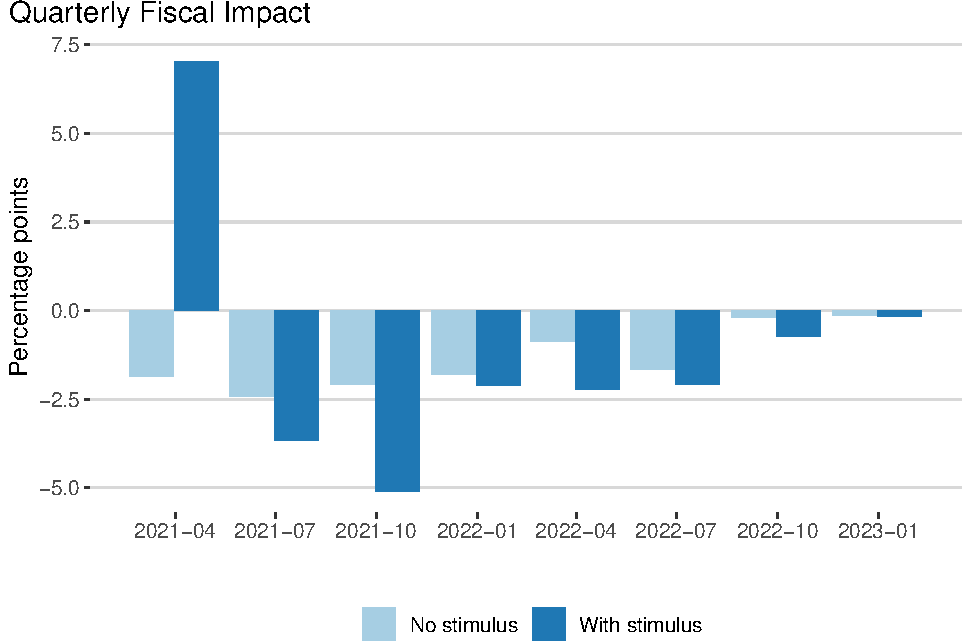
\includegraphics{stimulus-changes_files/figure-latex/fim-1} \end{center}

\begin{center}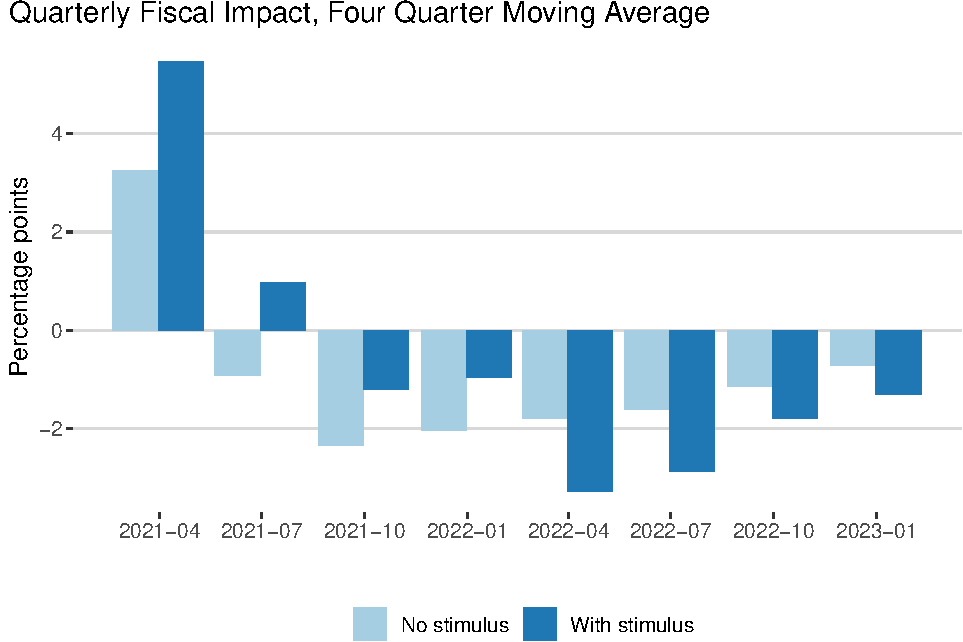
\includegraphics{stimulus-changes_files/figure-latex/fim-ma-1} \end{center}

\hypertarget{purchases-and-grants}{%
\subsection{Purchases and Grants}\label{purchases-and-grants}}

\begin{center}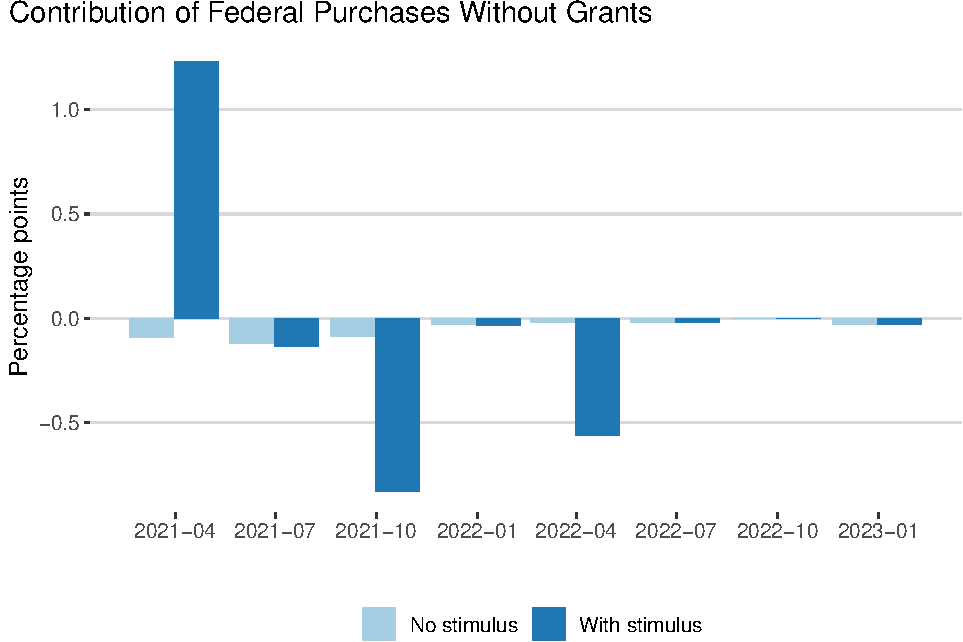
\includegraphics{stimulus-changes_files/figure-latex/purchases-federal-1} \end{center}

\begin{center}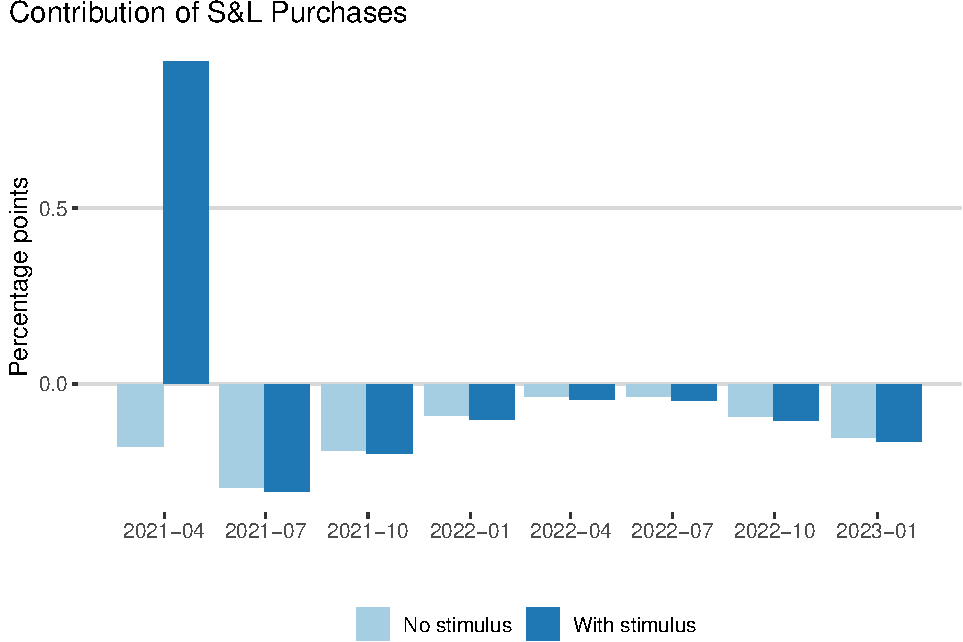
\includegraphics{stimulus-changes_files/figure-latex/purchases-state-1} \end{center}

\begin{center}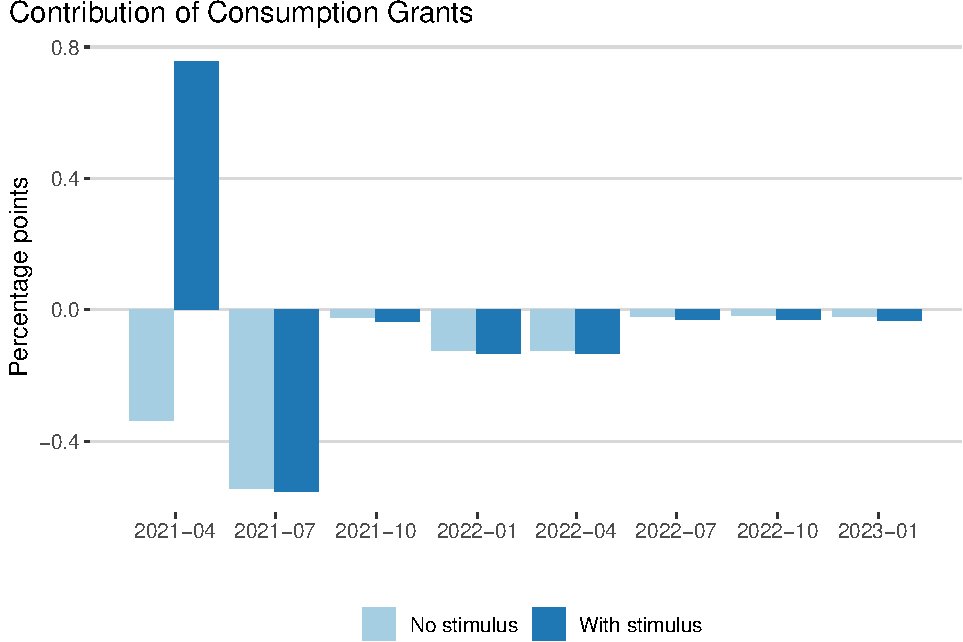
\includegraphics{stimulus-changes_files/figure-latex/cgrants-1} \end{center}

\begin{center}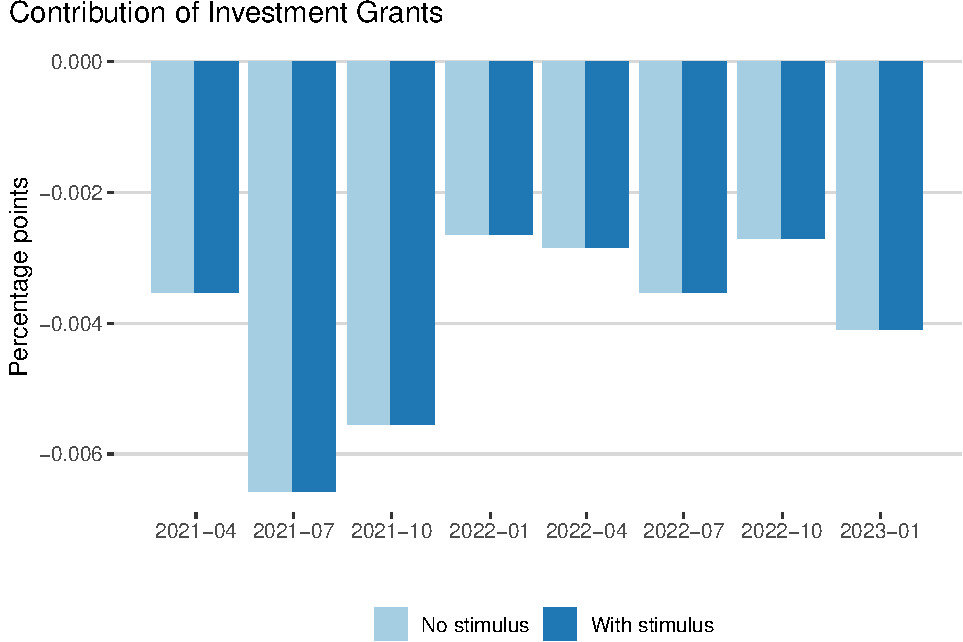
\includegraphics{stimulus-changes_files/figure-latex/igrants-1} \end{center}

\hypertarget{taxes-and-transfers}{%
\subsection{Taxes and Transfers}\label{taxes-and-transfers}}

\begin{center}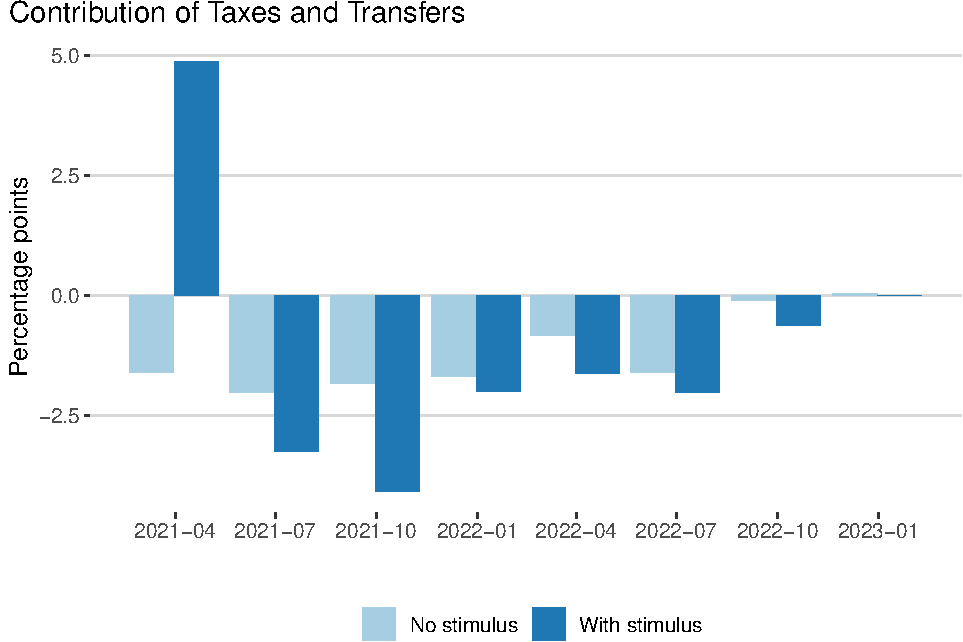
\includegraphics{stimulus-changes_files/figure-latex/tts-1} \end{center}

\begin{center}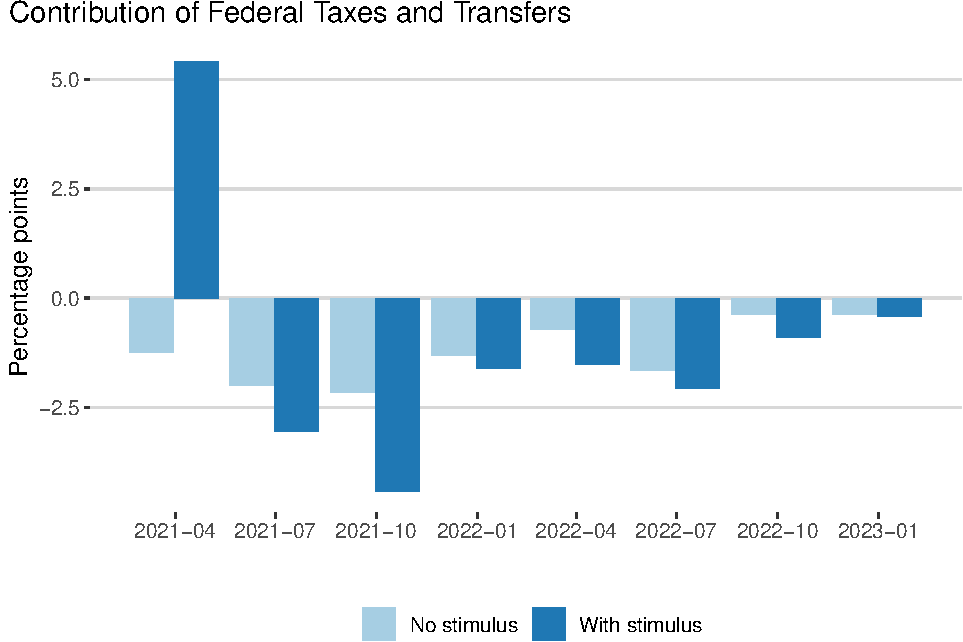
\includegraphics{stimulus-changes_files/figure-latex/federal-tts-1} \end{center}

\begin{center}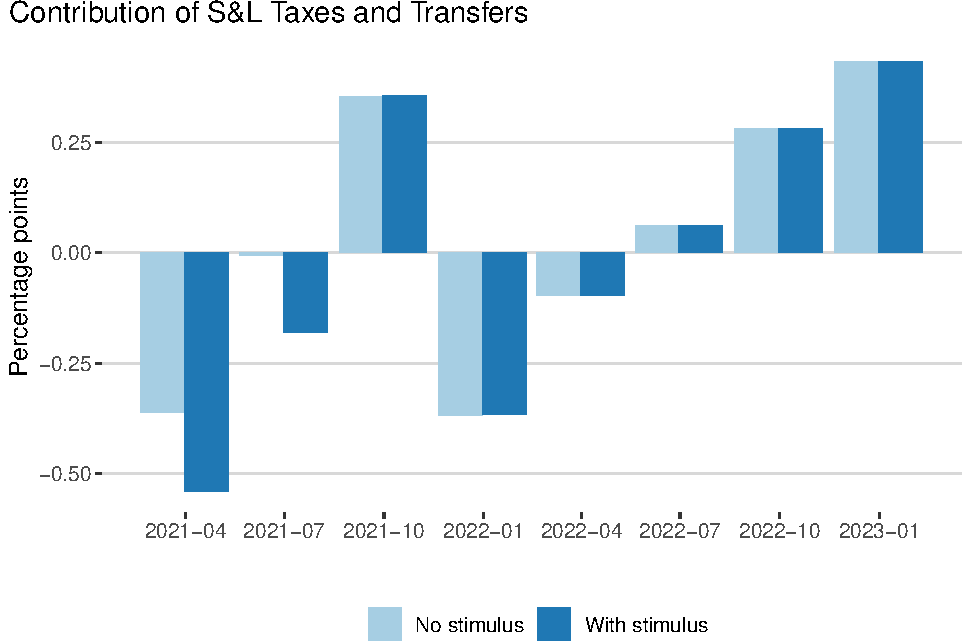
\includegraphics{stimulus-changes_files/figure-latex/state-tts-1} \end{center}

\hypertarget{subsidies}{%
\subsection{Subsidies}\label{subsidies}}

\begin{center}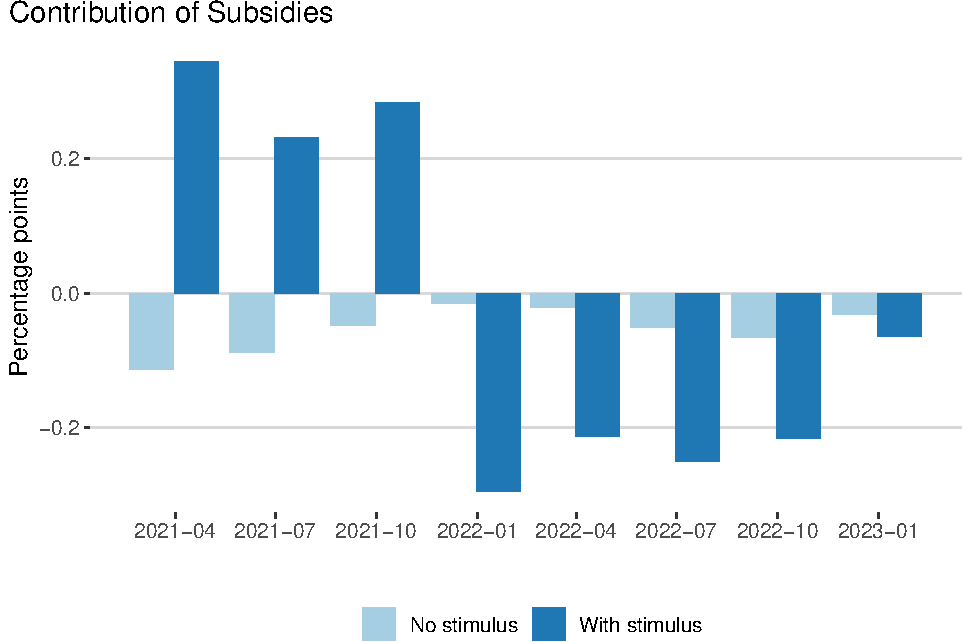
\includegraphics{stimulus-changes_files/figure-latex/subsidies-1} \end{center}

\begin{center}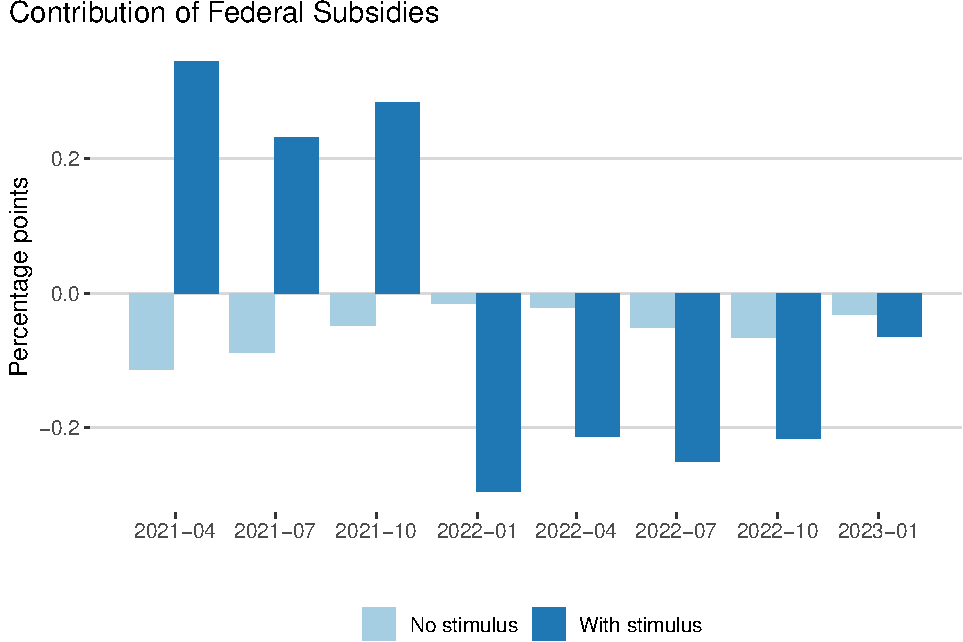
\includegraphics{stimulus-changes_files/figure-latex/subsidies_federal-1} \end{center}

\begin{center}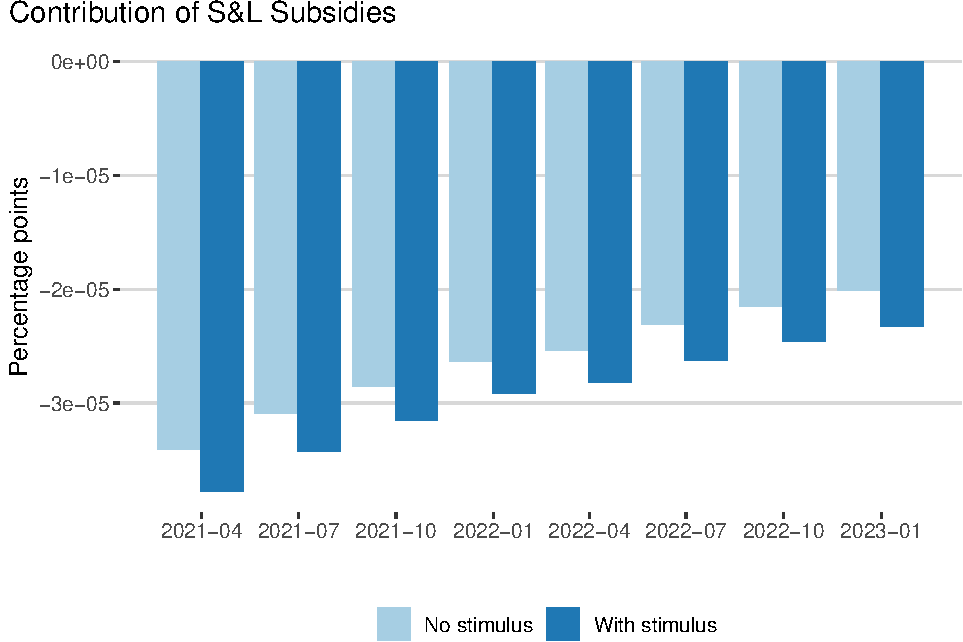
\includegraphics{stimulus-changes_files/figure-latex/subsidies_state-1} \end{center}

\begin{center}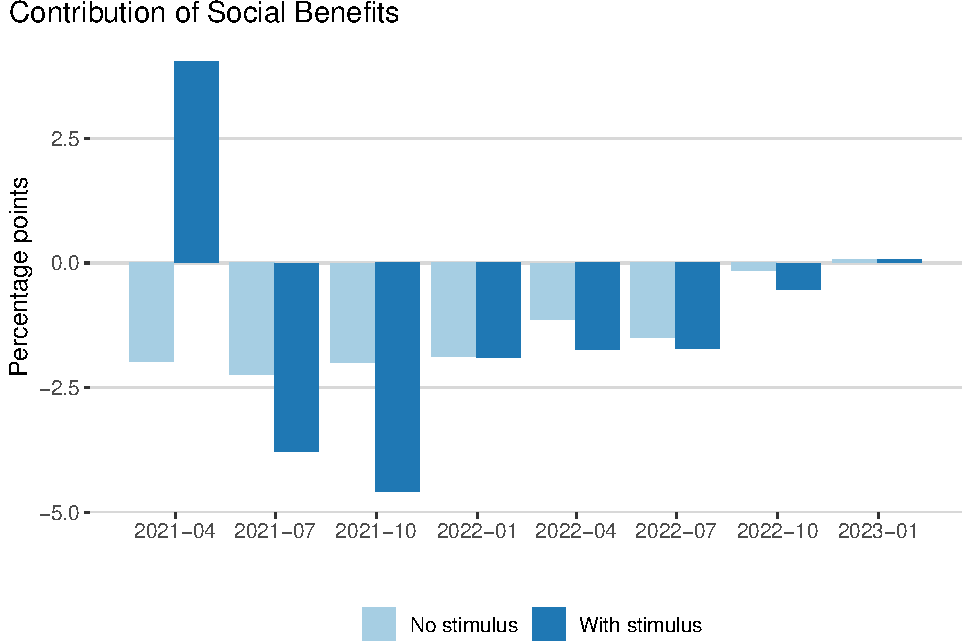
\includegraphics{stimulus-changes_files/figure-latex/social-benefits-1} \end{center}

\end{document}
